\section{Circuito de medición}
En la figura \ref{fig:circuito_completo} se presenta el diagrama del circuito completo, las partes del circuito se encuentran nombradas, en las siguientes secciones se dará una descripción de los mismas.
\begin{figure}[H]
\centering
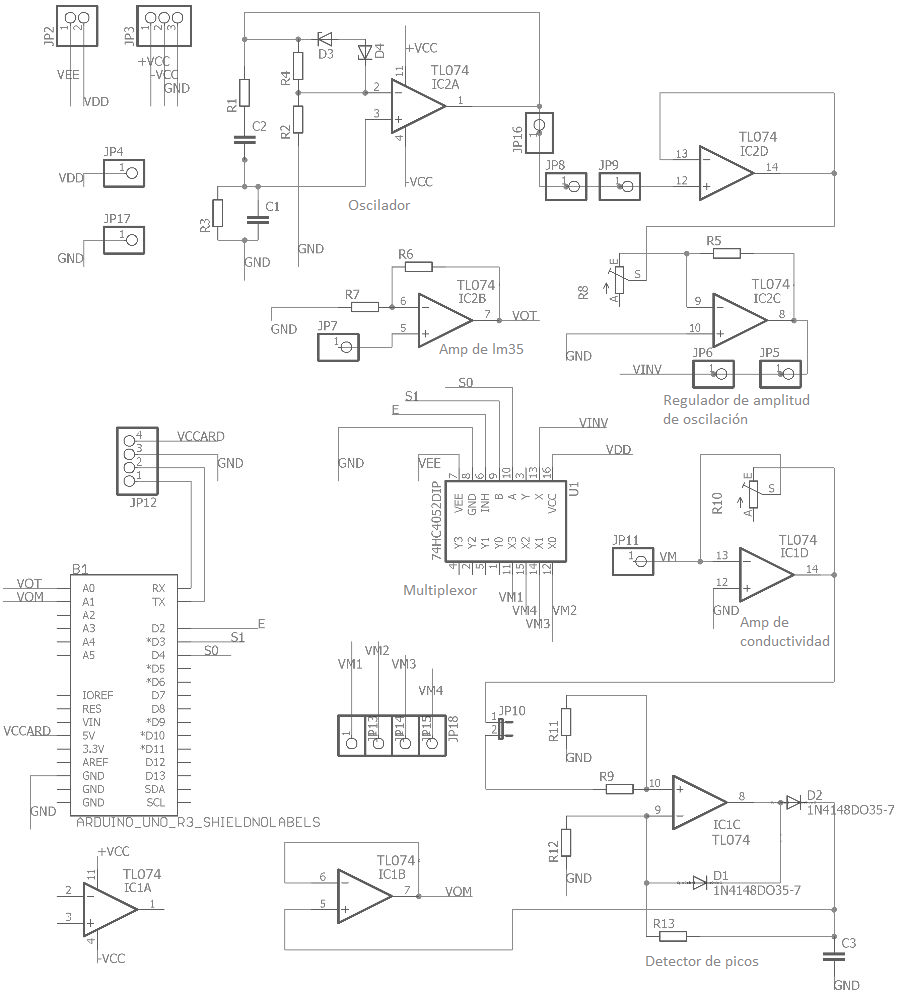
\includegraphics[width=1.1\textwidth]{circuito_completo.png}
\caption{Diagrama circuito completo}
\label{fig:circuito_completo}
\end{figure}

\section{Oscilador de Wien}
 \subsection{Diseño}
  El circuito correspondiente al bloque del Oscilador de Wien diseñado se representa en la figura \ref{fig:oscilador}.
  
 \begin{figure}[!htb]
\centering
\begin{tikzpicture}[scale=2]
\draw[color=black, thick][american voltages][american currents]

% NODO A TIERRA
(1,0) node[ground]{}

(1,0) to [R,l=$R_1$] (1,1)

%Amplificador
(2,1.5) node[ op amp ] (opamp) {}
(opamp.out) node[] {}
%----------DIVISOR DE R2 y R1--------------------------- % 
(opamp.+) node[] {}
(opamp.+)-| (1,1)
(1,1.25) to [R,l=$R_2$,*-o](-0.25,1.25)
(-0.25,1.25) node[left] {\Large $v_{in}$}
%-------------------------------------------------------- %
%----------Entrada INVERSORA--------------------------- --% 
(opamp.-) -| (1, 2.75)  to [D*,l_=$D_1$,v^>=$v_{D1}$, i_=$i_{D1}$,*-](3,2.75) |- (opamp.out)
(1,2.5) to (1,3.25) to [R,l=$R_4$](4.5,3.25) to (4.5,1.5)
(-0.25,1.75) to [R,l=$R_3$,-*](1,1.75) 
%----- ------NODO A TIERRA------------------------------- -%
(-0.25,1.75) node[ground, rotate=-90]{}
%--------------------------------------------------------- %
(3,1.5) to [D*,l_=$D_2$, v^>=$v_{D2}$, i_=$i_{D2}$,-*](4.5,1.5)
(4.5,0) to [C,l^=$C$,v_<=\Large $ v_{out}$](4.5,1.5)
% NODO A TIERRA
(4.5,0) node[ground]{}
% ------------- %
(opamp.-) node[above] {\Large $v^-$}
(opamp.+) node[above] {\Large $v^+$}

%---------Fuentes de alimentacion ------------------------- %
(opamp.up) --++ (0,0.1) node[above]{15\,\textnormal{V}}
(opamp.down) --++(0,-0.1) node[below]{-15\,\textnormal{V}}

;
%\draw[black,thick,dashed] (-0.45,1.9) rectangle (3.25,-0.35);

%\draw[black,thick,dashed] (-0.45,4.8) rectangle (3.25,2);
\end{tikzpicture}
\caption{Detector de picos}
\label{fig:detectorPicos}
\end{figure}

Si inicialmente no se considera la presencia de los diodos, se puede ver que el circuito de la figura \ref{fig:oscilador} se corresponde con un diagrama de bloques como el de la figura \ref{fig:DiagramaDeBloquesOscilador}. El bloque $A$ se corresponde con el recuadro superior de la figura \ref{fig:oscilador} y el bloque $\beta(s)$ se corresponde con el recuadro inferior de dicha figura.

% \documentclass{article}
\begin{figure}[H]
\centering
%\usepackage{tikz}
%\usetikzlibrary{shapes,arrows}
%\usepackage{verbatim}

 \tikzstyle{block} = [draw, fill=blue!20, rectangle, minimum height=3em, minimum width=5em]
 
 \tikzstyle{input} = [coordinate]
 
 \tikzstyle{output} = [coordinate]
 
 \begin{tikzpicture}[auto, node distance=2cm,>=latex']
 
 	\node [input, name=input] {};
 
 	\node [block, right of=input] (A) {\LARGE A};
 	
 	\node [output, right of=A] (output) {};
 	
 	
 	\node [block, below of=A] (BETA) {\LARGE $\displaystyle{\beta(s)}$};
 	
 	\node [output, left of=BETA] (outBeta) {};
 	
 	\draw (A) -- (output);
 	\draw [->] (output) |- node {\LARGE $v_{osc}$} (BETA);
 	
 	\draw (BETA) -- (outBeta);
 	\draw [->](outBeta)  |- node {\LARGE $v_f$} (A) 
 	
 	;
 	 	
 \end{tikzpicture}
\caption{ Diagrama de bloques del Oscilador}
\label{fig:DiagramaDeBloquesOscilador}
\end{figure}


El bloque $A$ es un amplificador no inversor de ganancia:
 $$A=1+\frac{R_2}{R_1}$$

 Por otro lado, el bloque $\beta(s)$ tiene una transferencia dada por:
\begin{equation*}
\beta(s)=\frac{\omega_n s}{s^2+3\omega_ns+\omega_n ^2} \hspace{0.5cm}donde\hspace{0.5cm} w_n=\nicefrac{1}{RC}
\end{equation*}

Abriendo el lazo a la entrada del bloque $A$, tendremos una transferencia en lazo abierto dada por:

$$A\times \beta(s) = \left( 1+\frac{R_2}{R_1}\right) \times \frac{\omega_n s}{s^2+3\omega_ns+\omega_n ^2} $$

Por criterio de Barkhausen, el circuito va a mantener oscilaciones en régimen únicamente a frecuencias $\omega$ para las cuales se cumplen las dos condiciones:

$$\textbf{(C1)}: \hspace{0.1cm}\arg\left(A\times \beta(j\omega)\right)=0$$
$$\textbf{(C2)}: \left| A\times \beta(j\omega)\right| =1$$

Evaluando la transferencia en lazo abierto en $s=jw$ tenemos:

$$A\times \beta(j\omega) = \left( 1+\frac{R_2}{R_1}\right) \times \frac{j\omega_n\omega}{(\omega_n ^2-\omega ^2) +3j\omega_n\omega} $$
La única frecuencia a la cual se puede cumplir la condición (C1) es $\omega= \omega_n$. Evaluando el módulo de la transferencia en lazo abierto en dicha frecuencia, obtenemos:
$$\left| A\times \beta(j\omega_n)\right|  = \left( 1+\frac{R_2}{R_1}\right)\times\frac{1}{3}$$
Solamente pueden cumplirse (C1) y (C2) a la vez si:
\begin{equation}
1+\frac{R_2}{R_1}=3
\label{eq:relacion3}
\end{equation}

Por tanto, se eligen $R_2$ y $R_1$ tales que $R_2=2R_1$.\\\\
Notamos que para $A=3$, la única forma de que funcione correctamente el lazo cerrado es con $s=jw_n$. Entonces el valor de la frecuencia de oscilación está dado por: 
$$f_n=\frac{1}{2\pi RC}$$

\subsubsection{Respecto a los diodos (EXPLICAR)}
{\color{red}  Se le agrega los diodos Zener EDZV27B y se cambia la resistencia $R_{2}$ por un potenciómetro para poder regular la amplitud de oscilación, de lo contrario la señal satura o se anula dependiendo de si se aproximó por arriba de 1 o por abajo  a la condición de Barkhausen.}\\
\label{secc:diodos}
\subsection{Componentes Seleccionados}


Para el bloque $\beta(s)$ se elijen los componentes observados en el cuadro \ref{tabla:componentesBeta}. Los mismos se elijen de manera tal que se obtenga una frecuencia del orden de los 10kHz. Con esto en mente, se seleccionan resistencias del orden de los ohmios para obtener capacidades del orden de los nano faradios, los cuales son valores estándar en el mercado local.

\begin{table}[htb]
		\tamano\centering
		\caption{Valores de las componentes para el bloque $\beta(s)$}
		\label{tabla:componentesBeta}
		\begin{tabular}{|l|l|l|l|}
			\hline
			$R$($\Omega$) & C(nF)  \\ \hline
			120 & 100 \\ \hline
		\end{tabular}
\end{table}    
    


En el caso del bloque A, se seleccionan dichos valores de resistencia debido a que se disponía de los mismos. Se utilizan los diodos EDZV27B por lo mencionado en la sección \ref{secc:diodos}.

\begin{table}[htb]
\centering
\caption{Valores de los componentes para el bloque A}
\label{tabla:componentesA}
\begin{tabular}{|l|l|l|l|}
\hline
$R_1$(k$\Omega$) & $R_2$(k$\Omega$) & Amp. Op. & Diodos \\ \hline
10 & 20 & Tl071    & EDZV27B \\ \hline
\end{tabular}
\end{table}
\subsection{Simulación del circuito en \emph{LTSpice}}

 Se gráfica la simulación del voltaje $v_{osc}$  en régimen en función del tiempo. Dicha gráfica se puede ver en la figura \ref{sim:Vosc}. 

\begin{figure}[H]
	\centering
	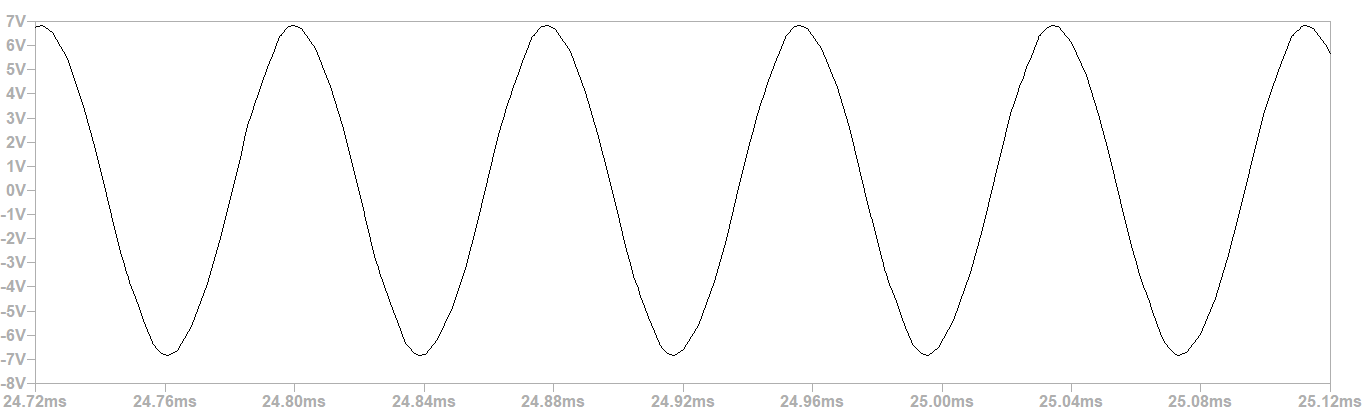
\includegraphics[width=0.9\textwidth]{Oscilador/salida_simulada.png}
	\caption{Simulación: Voltaje de salida del oscilador}
	\label{sim:Vosc}
\end{figure}
El valor teórico de la frecuencia de oscilación está dado por: 
$$f_n=\frac{1}{2\pi RC}\Longrightarrow f_n = 13,262 \si{\kHz}$$
El voltaje de salida $V_{osc}$ simulado resultó ser una onda senoidal.\\
de frecuencia:
$$f_n^{sim}=12.41 kHz$$
y amplitud:
$$V_o^{sim} =  6.84 V$$
%Esto sirve porque, para evitar efectos de polarización de los electrodos de la celda de medida de conductividad, se desea trabajar a frecuencias cercanas a $10\si{\kHz}$.
\subsection{Implementación (Pendiente)}
VER QUE PASÓ AL IMPLEMENTARLO Y ANOTAR COSAS Y COMPARAR.





